\section{The inner Galactic landscape} \label{sec:IG}

The CMZ\index{Central Molecular Zone} is not an isolated system. It is in a constant state of flux due to the inflow of matter from the Galactic disc. Understanding how stars and planets form in this environment requires an understanding of the dynamic landscape within which the CMZ is set. We therefore begin our review with a taxonomy of the inner Galaxy, its key components, and the dynamical features that provide essential context for our understanding of star formation in this environment. 

\subsection{Mapping the landscape: dynamical features observed in the cold ISM} \label{sec:cartography}

The centre of the Milky Way has been extensively mapped across the electromagnetic spectrum for over half a century. Observations of H\,{\sc i} in the 1950s and 60s unveiled its complex dynamics, shaping our understanding of the large-scale structure of the Milky Way \citep[e.g.][]{Oort1958,Rougoor1960,deVaucouleurs1964}. Later, observations of CO in the 1970s and 80s, free from the confusion in H{\sc i} due to the near-ubiquity of atomic gas along the line-of-sight, delineated the structure of the molecular gas associated with the CMZ \citep{Bania1977, Liszt1978, Bally1987}. For extensive discussion on the history of these observations we recommend the reviews by \citet{Oort1977}, \cite{Combes1991}, and \citet{Morris1996}, and for a more recent update, \citet{Bryant2021}. In the following sections, we describe several of the key features of the inner Galaxy that are foundational to our understanding of the origin of the CMZ and the star formation occurring within it. We highlight these features in Fig.~\ref{fig:lbv_main}, which depicts the distribution of molecular gas within  $|l|<10^{\circ}$ as it appears on the plane of the sky in longitude-latitude, $\{l,b\}$ space as well as in longitude-velocity, $\{l,v\}$ space.

\subsubsection{The dust lanes}\label{sec:dustlanes}

A key component of the star formation process in the Galactic Centre is the inflow from kiloparsec scales. We will discuss the theoretical understanding of the inflow process in \S\ref{sec:generaldynamics} and quantify the inflow rate towards the centre of the Milky Way in \S\ref{sec:barinflow}. Here, we deal with the observational manifestation of the inflow process in the Milky Way: the inner Galactic dust lanes. 

The dust lanes\index{Galaxy!dust lanes} associated with galactic bars can be clearly seen in images of face-on spiral galaxies \citep{Sandage1961,Knapen2002, Comeron2009, Lee2022}. However, our embedded view through the Galactic plane makes identifying the Milky Way's dust lanes more challenging. The identification of the features believed to correspond to the Milky Way's dust lanes has therefore mostly relied on the emission from spectroscopic data (often H\,{\sc i} and CO observations) viewed in $\{l,v\}$-space, such as the diagrams shown in the lower panels Fig.~\ref{fig:lbv_main} \citep[e.g.][]{Fux1999}. The name ``dust lanes'' has been retained for historical reasons, though they have also been subsequently identified in three-dimensional dust extinction maps \citep{Marshall2008}. The two ``primary'' dust lanes are marked in Fig.~\ref{fig:lbv_main} as the near and far side lanes, respectively, and are further highlighted in the face-on schematic presented in Fig.~\ref{fig:sketch}. The near side dust lane is readily identified in H{\sc i} emission, and was originally dubbed the ``connecting arm'' \citep[][]{Cohen1976, McClure-Griffiths2012}. The vast majority of the emission associated with the near (far) side dust lane is located at positive (negative) longitudes and velocity, and negative (positive) latitudes, respectively, although note that the far side dust lane does extend to positive velocity \citep[][]{Fux1999, Liszt2006, Liszt2008, Rodriguez-Fernandez2006, Sormani2019b}. The detection of the dust lanes in opposite quadrants in $\{l,b\}$ suggests that they lie on a common plane that is tilted with respect to the Galactic plane by $\sim2\mhyphen3^{\circ}$ \citep{Sormani2019b,Tress2020}. A tilt of the inner Galactic gas layer is also observed in the ionised and neutral gas \citep[e.g.][]{Krishnarao2020b}. A secondary family of less prominent and less extended dust lanes that are roughly parallel to the primary dust lanes in the $\{l,v\}$ plane, was identified by \citet{Liszt2008}. Two of these secondary dust lanes are highlighted in Fig.~\ref{fig:lbv_main}. These secondary dust lanes have been interpreted as shorter lane segments parallel to the main dust lanes in real space \citep[Fig.~\ref{fig:sketch};][]{Rodriguez-Fernandez2006,Sormani2019a}. 

\subsubsection{Extended velocity features}\label{sec:EVFs}

Another phenomenon that may be related to the inflow process from kiloparsec scales is a class of object that we will refer to as Extended Velocity Features (EVFs; \citealp{Sormani2019a}). EVFs are immediately identifiable in the $\{l,v\}$ diagram as near-vertical features (Fig.~\ref{fig:lbv_main}). We distinguish EVFs from another class of features known as High Velocity Compact Clouds (HVCCs, not to be confused with HVC or High Velocity Clouds found in the halo of the Milky Way, e.g.~\citealt{Wakker1997}), despite some overlap in the original classification \citep[HVCCs are similar in that many appear as near-vertical emission features in $\{l,v\}$ diagrams;][]{Oka1998b}. HVCCs have been speculated to be associated with phenomena such as supernova explosions \citep{Oka1999} and even with the presence of intermediate-mass black holes \citep[IMBHs;][]{Oka2016, Oka2017, Takekawa2017b, Tokuyama2019}. In contrast, the connection (in $\{l,b,v\}$-space) between EVFs and the dust lane features described above implies a physical connection between the two \citep{Liszt2008}, indicating that EVFs more likely result from larger-scale dynamical processes. The most prominent of the EVFs are highlighted in Fig.~\ref{fig:lbv_main} at $l\approx5.4^{\circ}$ and $l\approx3.2^{\circ}$. This latter feature is also known as Bania's Clump 2 \citep{Bania1977}. It has a total velocity extent of the order $\sim150$\,\kms \ \citep{Stark1986, Longmore2017}. Similar features appear at $l\approx1.3^{\circ}$, $-0.5^{\circ}$, and $-1.0^{\circ}$ \citep{Liszt2006}. Generally, the EVFs are compact in longitude, but can be extended in latitude \citep[in some cases by over 100\,pc;][]{Liszt2006}. Their velocity extents can be as large as 200\,\kms. 

Following their discovery, EVFs were interpreted as streams of clouds falling into the CMZ \citep{Stark1986, Boyce1989, Baba2010}. However, \citet{Stark1986} acknowledged that this explanation relies on the near-perfect line-of-sight alignment of the clouds (the so-called ``fingers of God'' effect). A more recent interpretation, which has emerged thanks to the advancement of numerical simulations that describe the flow of gas in a barred potential (\S\ref{sec:generaldynamics}), is that the EVFs represent the rapid deceleration of gas resulting from collisions between gas travelling along the dust lanes towards the CMZ and either: 1) gas that was formerly travelling along the opposite dust lane but has `overshot' the CMZ; 2) gas that belongs to the CMZ itself \citep{Fux1999, Liszt2006, Liszt2008, Rodriguez-Fernandez2008, Bally2010, Sormani2019a, Akhter2021}. This interpretation naturally explains the apparent association between the EVFs and the inner Galactic dust lanes (\S\ref{sec:dustlanes}), and further explains why no known EVF extends beyond the terminal velocity curve at its observed Galactic longitude \citep{Sormani2019a}. That said, the EVFs have been broadly interpreted.  An alternative view is that the EVFs represent the footprints of ``giant molecular loops'' generated by the Parker instability \citep{Parker1966}. These footprints are speculated to be characterised by large velocity gradients and strong shocks caused by gas that is accelerated along magnetic field lines due to gravity, colliding with the Galactic plane \citep{Fukui2006, Fujishita2009, Machida2009, Torii2010, Kakiuchi2018, Riquelme2018, Enokiya2021}. They have also been suggested to arise from collisions between the gas in the CMZ and an expanding ring of molecular gas \citep{Uchida1994,Oka2020}, driven by an explosive event near the centre of the Galaxy (see \S\ref{sec:cmz}). 

\subsubsection{The Central Molecular Zone}\label{sec:cmz}

``The CMZ''\index{Central Molecular Zone} is the concentration of molecular material observed within Galactocentric radius $R\simeq300$\,pc \citep[][]{Morris1996}. In CO emission, the CMZ is brightest over the inner $\sim4^{\circ}$ \citep{Bally1988, Oka1998b, Eden2020}. However, the gas distribution is asymmetric about the Galactic centre\index{Galaxy!Center}, with roughly three-quarters of the emission located at positive Galactic longitudes and velocities (see the right panels of Fig.~\ref{fig:lbv_main} and \S\ref{sec:gasstardistrib}). The total mass of molecular gas within $R\simeq300$\,pc is estimated to be $2\mhyphen6\times10^{7}$\,\msun \citep{Dahmen1998, Ferriere2007}. This corresponds to $3\mhyphen10\%$ of all the molecular gas in the Galaxy \citep[$6.5\times10^{8}$\,\msun; ][]{Roman-Duval2016} despite only accounting for $0.1\%$ of the surface area. 

Historically, the CMZ has been divided into two main components \citep{Morris1996,Fux1999}. Each component is distinguishable by its mass and kinematics, and we describe each of them below. 

\begin{figure*}
    \centering
	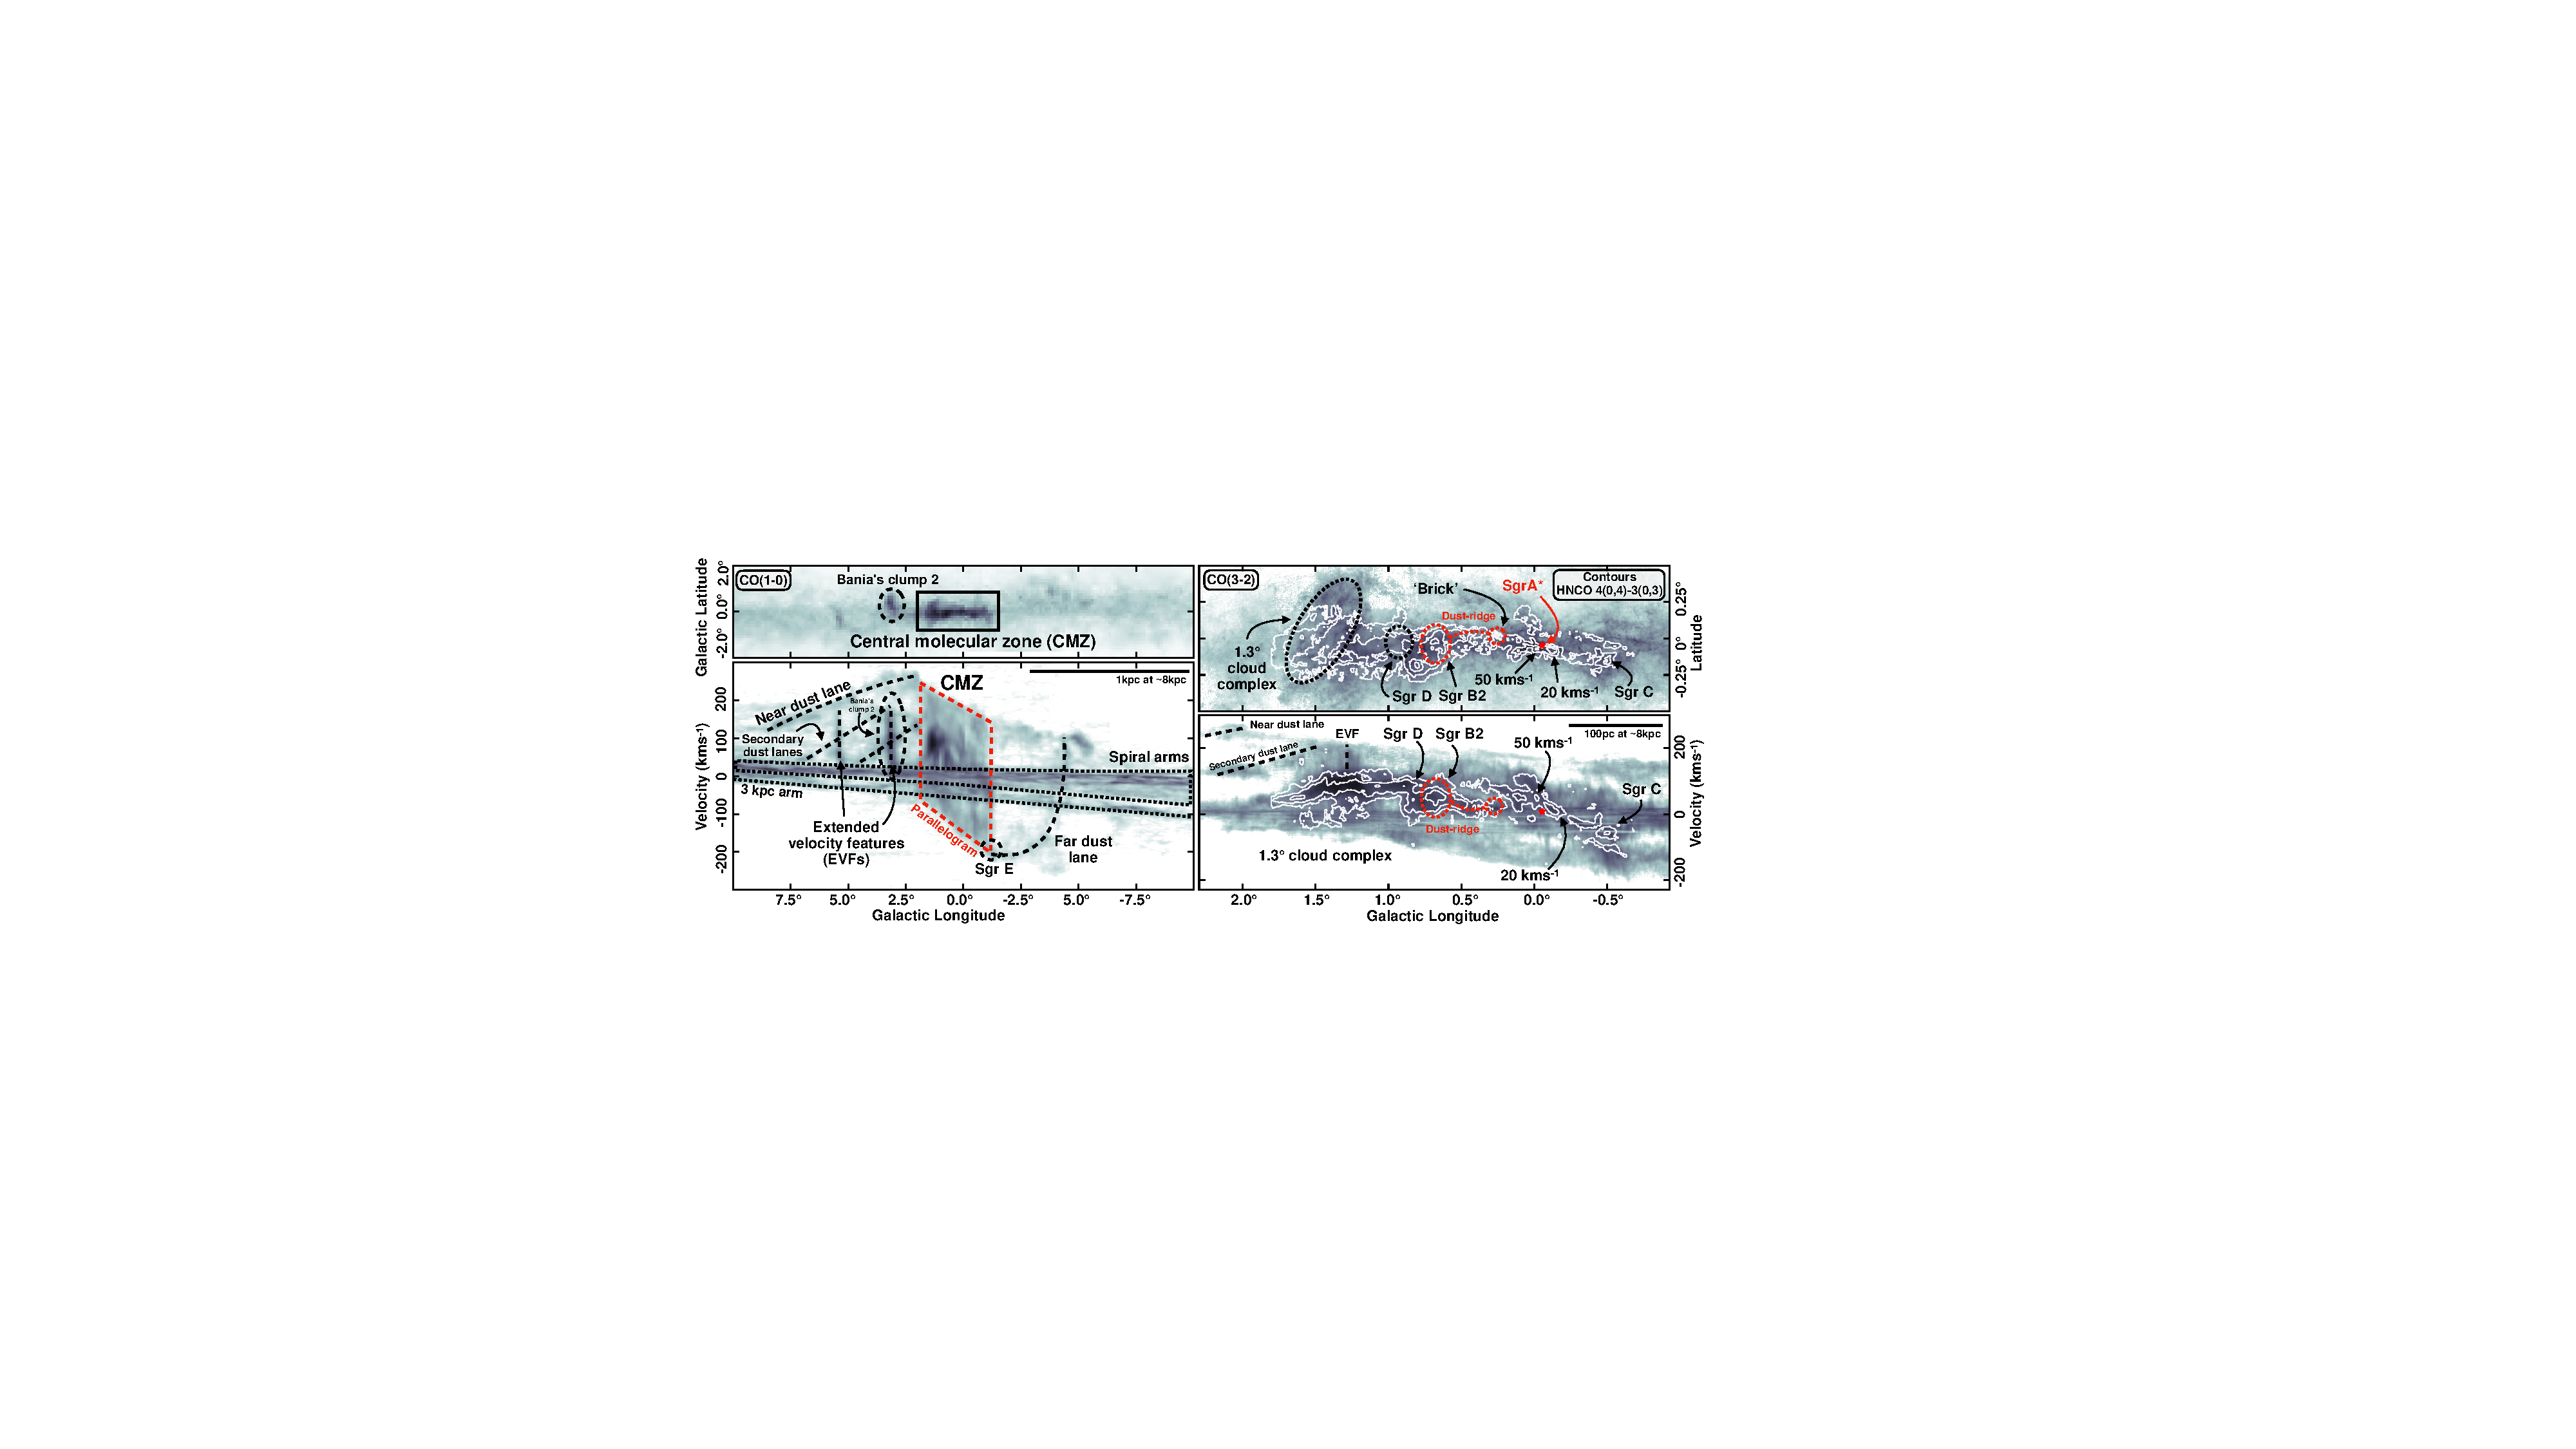
\includegraphics[trim=0 0cm 0 0cm, clip, width=0.9\textwidth]{./figs/lbv_compressed_v3.pdf}
    \caption{Atlas of the position-position-velocity ($\{l,b,v\}$ space) structure within the centre of the Milky Way. 
    The left panels show the integrated intensity of the $^{12}$CO $J=1-0$ line across the central few degrees ($\sim\,$ few kpc) of the Galaxy \citep{Dame2001}.
    The right panels show the integrated intensity of the $^{12}$CO $J=3-2$ line across the inner degree ($\sim\,$~300\,pc) taken as part of the CHIMPS2 survey \citep{Eden2020}.
    Overlaid as white contours is the HNCO\,$4(0,4)\mhyphen3(0,3)$ emission, a tracer of denser gas, taken as part of the Mopra CMZ survey \citep{Jones2012}.
    Labelled on both sets of panels are the prominent features discussed throughout this review (see in particular \S\ref{sec:IG} for the taxonomy of the inner Galaxy, and \S\ref{sec:massreservoir} for a detailed discussion of structures in the CMZ). The horizontal stripes in the CO emission shown in bottom-right panel are absorption from foreground spiral arms.}
    \label{fig:lbv_main}
\end{figure*}
 
\paragraph{The $\{l,v\}$ parallelogram vs. the ``expanding molecular ring''.}\label{subsubsec:180pcring} The first of the two components associated with the CMZ has been broadly interpreted. It is recognisable in $\{l,v\}$-space as a parallelogram-shaped feature (highlighted in Fig.~\ref{fig:lbv_main}). It traces highly non-circular motions\index{galaxies!kinematics and dynamics} between $-1.3^{\circ}\lesssim l \lesssim 2.0^{\circ}$, $b=0.0^{\circ}$ and $|v|\lesssim250$\,\kms. 

The original interpretation of this feature was that it represents a radially expanding ring of molecular gas \citep[sometimes referred to as the expanding molecular ring, EMR, or the ``$180$\,pc expanding ring'';][]{Scoville1972, Kaifu1972, sofue1995b, Oka2020}, although the geometry has evolved over time \citep{Sofue2017a}. It has been speculated that the EMR is driven by some highly energetic and expansive event (or a combination of events) occurring near the centre, namely extensive central star formation activity, many supernovae, or past activity from the central supermassive black hole, Sgr\,A* \citep{Sofue2017a}. 

There are two main persistent criticisms of this interpretation. First, the required energy input is very high. The molecular gas mass of the EMR is $\sim0.5\mhyphen1.0\times10^{7}$\,\msun, which, when combined with the estimated expansion velocity of $160$\,\kms, corresponds to a kinetic energy of $10^{54}\mhyphen10^{55}$\,erg \citep[roughly the equivalent of $10^{3}\mhyphen10^{4}$ supernovae][]{Scoville1972, sofue1995b, Sofue2017a, Oka2019}. Second, while there is evidence for outflows being driven vertically out of the Galactic plane from the central region \citep[][see \S\ref{sec:feedback}]{Bland-Hawthorn2003, Su2010, Heywood2019, Heywood2022}, there is little direct evidence for any in-plane impact of such an event \citep[][]{Combes1991}.

The more widely accepted interpretation of the parallelogram is that it arises in the context of the non-circular motions driven by the Galactic bar (see \S\ref{sec:generaldynamics}). This interpretation is attractive in that it does not need to invoke a large-scale expansive event, nor does it require ad-hoc assumptions since the presence of the Galactic bar is well established. However, the details have significantly evolved over time. \citet{Binney1991} initially interpreted the parallelogram as the result of gas following the self-intersecting ``cusped'' $x_1$ orbit (a type of elongated orbit that exists in bar potentials; \S\ref{sec:generaldynamics}). However, we now know that the Galactic bar is much larger than hypothesised by \cite{Binney1991}, and, as a consequence, the cusped orbit is located at a much larger Galactocentric radius than in their model (\S\ref{sec:potential}). Recent numerical simulations have helped to refine this scenario. The key modification is that the gas associated with the parallelogram does not trace the cusped orbit \citep[][]{Fux1999, Sormani2018b}. Instead, the parallelogram can be understood in the context of the dust lanes described above (\S\ref{sec:dustlanes}). As the dust lanes deliver gas to the central region, not all of this gas will merge directly with the CMZ. Recent simulations have demonstrated that as much as 50-70\% of the infalling gas can overshoot the CMZ \citep{Hatchfield2021}. When observed in $\{l,v\}$-space, the gas overshooting the CMZ populates the top and bottom of the parallelogram (and some of the emission connected to it). 
The lateral sides of the parallelogram represent EVF-like features caused by the rapid deceleration of gas following the dust lane that is colliding with either gas in the CMZ itself or with gas located on the opposite dust lane.

\paragraph{``The CMZ'':}\label{subsubsec:cmz} The second component is mass-dominant, and is typically what we think of when we refer to ``the CMZ''. It is enclosed within the parallelogram described above. A map of this gas is shown in the right panels of Fig.~\ref{fig:lbv_main}, along with the corresponding $\{l,v\}$ diagram. For the remainder of this review, we make a distinction between this mass-dominant component, which we will henceforth refer to as ``the CMZ'', and the dust lanes described above and in \S\ref{sec:dustlanes}. The mass-dominant component extends over a Galactic longitude range of $-1.0^{\circ}\lesssim l \lesssim 1.7^{\circ}$, $|b|\lesssim0.5$, and $|v|\lesssim 150$\,\kms, and includes all of the major Galactic centre cloud complexes (Fig.~\ref{fig:lbv_main}): the 1.3$^{\circ}$ cloud complex, the so-called ``dust ridge'' clouds (including Sgr\,B2, G0.253+0.016 or ``the Brick'', and the clouds in between), the Sgr\,A clouds (consisting of the 20 and 50\,\kms \ clouds), and Sgr\,C. 
We further introduce here what we will refer to throughout the text as the ``100\,pc stream'' \citep{Kruijssen2015}. The 100\,pc stream contains all of the aforementioned clouds except for the $1.3^{\circ}$ complex. The 100\,pc stream is of particular interest for this review since it happens to be where the vast majority of present-day star formation is occurring (\S\ref{subsec:SFR:current}). The distinction between ``the CMZ'' and the ``100\,pc stream'' has been made in several works seeking to describe the 3D geometry of gas in the Galactic Centre \citep[\S\ref{sec:3d};][]{Rodriguez-Fernandez2006, Bally2010, Molinari2011, Kruijssen2015, Henshaw2016a}. However, the 3-D geometry of the CMZ remains unclear, and the $1.3^{\circ}$ cloud complex is a particular point of contention. This uncertainty is highlighted in Fig.~\ref{fig:sketch}, where we show schematic representations of the top-down view of the CMZ. For the purposes of this discussion, we shall state simply that the general consensus is that the gas in the CMZ is organised into a ring-like structure, the precise details of which are uncertain. We will revisit this topic, and the models presented in Fig.~\ref{fig:sketch}, in \S\ref{sec:macroevolution}.

\subsubsection{The circumnuclear disc}\label{sec:cnd} 

The final feature that we wish to discuss here is the circumnuclear disc\index[obj]{circumnuclear disc} (hereafter, CND). It remains uncertain how the CND relates to the larger scale features described above, but it is important in that it is the closest large reservoir of molecular gas to the central supermassive black hole Sgr\,A*\index[obj]{Sagittarius A*} \citep{Genzel1985,Guesten1987, Jackson1993}.  
It has an inner radius of $\sim1\mhyphen1.5$\,pc and an outer radius of $3\mhyphen7$\,pc, filling a ring-like structure with total mass $\sim3\times10^4$ \msun and densities $n\sim10^5\mhyphen10^7$\,cm$^{-3}$ \citep{Etxaluze2011,Oka2011,Mills2013,Tsuboi2018}. 
The exact mechanism by which gas is transported from the CMZ to the inner $10\mhyphen20$ parsecs is an open question (\S\ref{sec:inwardmassflow}). 
However, there is some evidence that the CND is built up from the tidal disruption of molecular clouds located within the inner $\sim10\mhyphen20$\,pc \citep{Ho1991,Coil2000, McGary2001, Martin2012,Mapelli2016,Hsieh2017,Hsieh2019, Tsuboi2018, Ballone2019}. 
Several filamentary molecular gas structures, or ``streamers'', have been detected surrounding the CND. These streamers have spatial extents $\sim$2\,pc and are speculated to act as channels that deliver gas to the CND \citep{Montero-Castano2009, Hsieh2017, Takekawa2017b}, possibly connected to ambient gas clouds located at a Galactocentric radius of 20\,pc (namely the Sgr\,A clouds; see \S\ref{sec:macroevolution}). 

The conditions found in the CND are extreme, even by CMZ standards.
The gas is highly excited, with most gas exceeding $T>500$ K and dust temperatures $\gtrsim 100$ K \citep{Bradford2005,Lau2013,Mills2013,Mills2017a,James2021}. The gas also exhibits extremely broad line-widths of $10\mhyphen40$\,\kms, reflecting a combination of high temperatures, elevated levels of turbulence\index{interstellar medium!turbulence} \citep{Goicoechea2018, Tsuboi2018, Hsieh2021}, and considerable rotational velocity\index{interstellar medium!kinematics and dynamics} ($\sim100$\,\kms). 
Contrasting measurements of the gas density have led to conflicting views on whether the gas is gravitationally bound or not \citep{Christopher2005, Montero-Castano2009, Requena-Torres2012}. 
It has been suggested that the CND is forming stars based on the detection of water and shock-excited methanol masers\index{masers}, candidate outflows traced by SiO (5-4), and compact, highly-excited and broad linewidth SiO emission interior to the CND \citep{Yusef-Zadeh2013a,Yusef-Zadeh2015b}. 
However, other explanations for these signatures exist and conclusive evidence of ongoing star formation in the CND is still lacking \citep{Mills2017a}.

\begin{figure}[!t]
    \centering
 	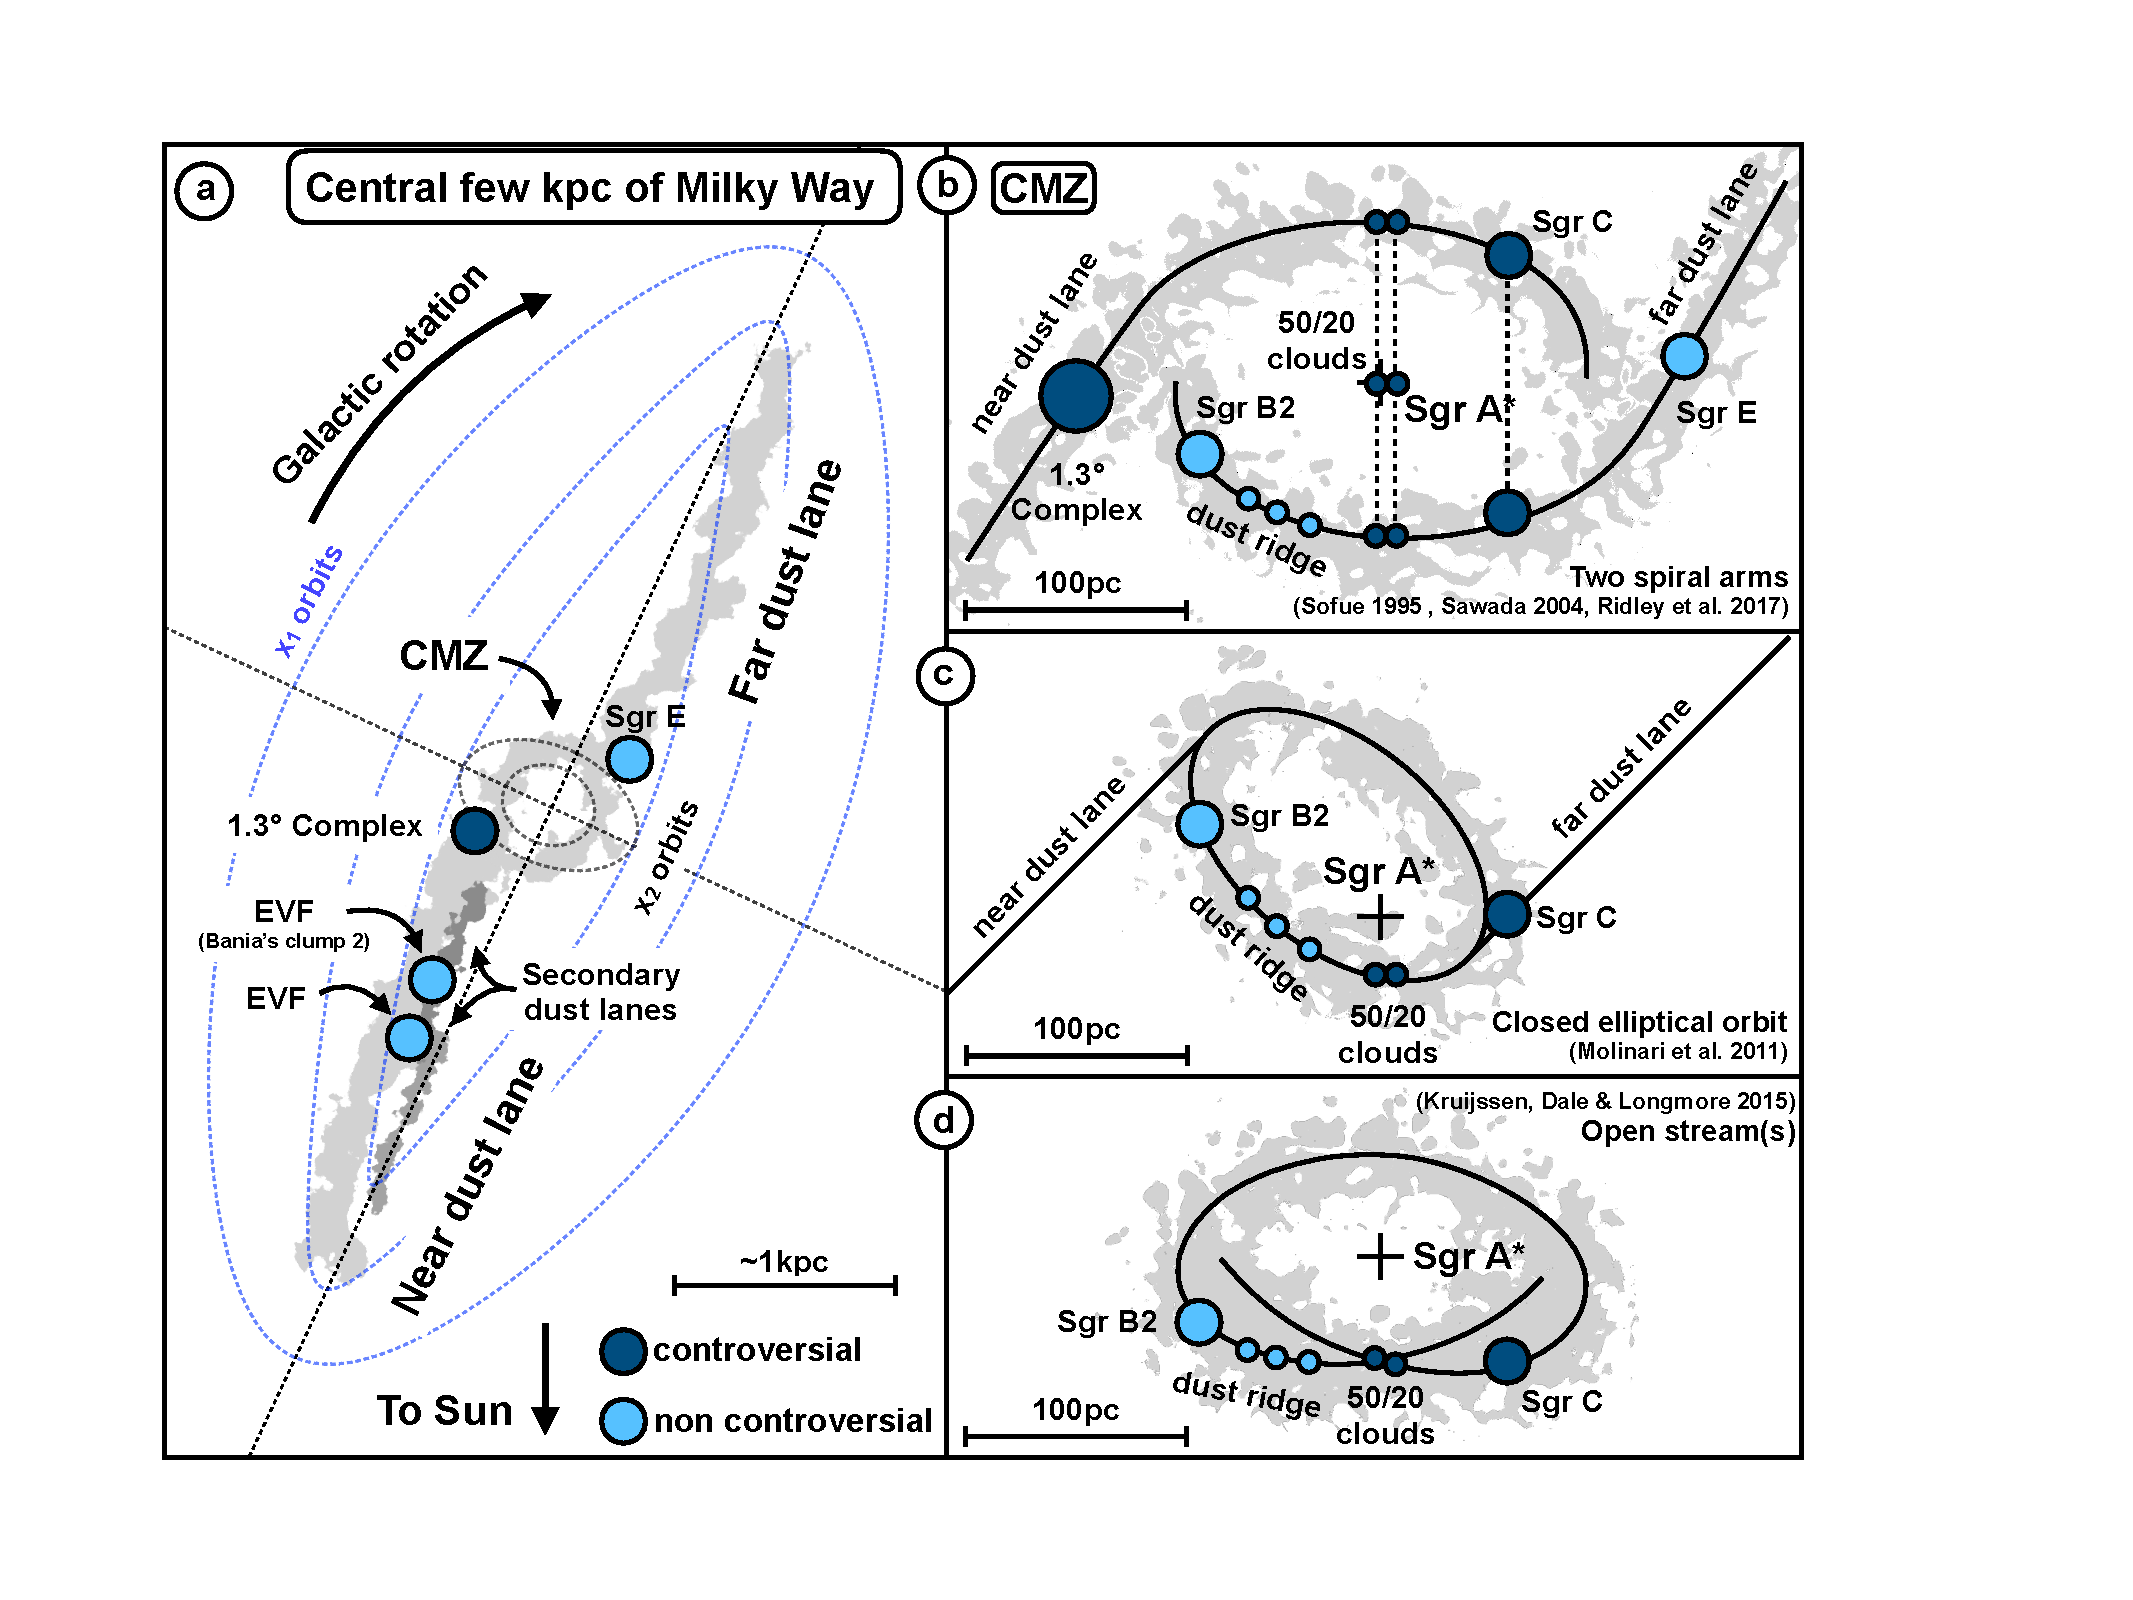
\includegraphics[trim=2.5cm 2.cm 5cm 2.cm, clip, width=1.0\columnwidth]{./figs/sketch.pdf}
    \caption{Schematic face-on view of the Galactic centre. On the left is a schematic of the inner few kiloparsecs of the Galaxy. It shows the dust lanes, EVFs, and CMZ discussed in \S\ref{sec:cartography}. Also included are the two main families of orbits ($x_1$, $x_2$) in a barred potential (\S\ref{sec:generaldynamics}). On the right are three different interpretations for the geometry of the CMZ. These are discussed in detail in \S\ref{sec:3d}. The features shown here are also labelled in Fig.~\ref{fig:lbv_main}. }
    \label{fig:sketch}
\end{figure}


\subsection{The origin of the CMZ} \label{sec:generaldynamics}

The very existence of the CMZ is a direct consequence of the inflow driven by the Galactic bar. The gravitational potential of the bar, and of the other components in the Galactic Centre, controls the size of the CMZ, influences the distribution, structure, and evolution of molecular clouds, and may help to create preferred locations for star formation. 
This section reviews our current understanding of the origin of the CMZ\index{galaxies!kinematics and dynamics}, and provides theoretical context to interpret the key observational features described in \S\ref{sec:cartography}. 

\subsubsection{The gravitational field in the inner Galaxy} \label{sec:potential}

The potential in the inner Galaxy\index{Galaxy!gravitational potential} is dominated by the following components in order of increasing Galactocentric radius of influence: (i) The central black hole Sgr A*\index{Sagittarius A*}. This generates a Keplerian potential with a mass of $M=4.15 \times 10^6\,\msun$ \citep{Ghez2008, Gillessen2009, GravityCollaboration2019} that dominates gravity in the central parsec ($R\lesssim 1\pc$); (ii) The nuclear stellar cluster\index[obj]{Nuclear Star Cluster} (NSC). The NSC is a dense, massive ($M \simeq 2.5 \times 10^7\, \msun$) and slightly flattened assembly of stars centred on Sgr\,A$^{*}$ \citep{Genzel2010,Schodel2014b,Feldmeier-Krause2017}. It dominates the potential in the range $1<R\lesssim30\,\pc$; (iii) The nuclear stellar disc\index[obj]{Nuclear Stellar Disk} (NSD). This is a flattened stellar structure with a mass of $M\simeq 1.05 \times 10^9\, \msun$ \citep{Launhardt2002,Sormani2020a, Sormani2021} that dominates the potential at Galactocentric radii $30 \lesssim R \lesssim 300\pc$. The NSD is co-spatial with the CMZ and generates most of the background gravitational field in which the gas in the CMZ flows. This co-spatiality is probably not coincidental. Gas in the CMZ and stars in the NSD rotate with similar velocities \citep{Schonrich2015,Schultheis2021}, and star formation in the CMZ contributes to the build-up of the NSD over secular timescales \citep{Baba2020}. Current observational constraints are consistent with the NSD being axisymmetric \citep{Gerhard2012,Valenti2016,Sormani2021}, although it cannot be ruled out that it is a nuclear bar \citep{Alard2001,Rodriguez-Fernandez2008}. Collectively, Sgr A*, the NSC and the NSD are often referred to as the nuclear bulge \citep{Launhardt2002}.

Finally, as with roughly 2/3 of all spiral galaxies in the local universe, the Milky Way hosts a stellar bar \citep{Blitz1991,Wegg2013}. The Galactic bar\index[obj]{Galactic bar} is a strongly non-axisymmetric structure whose major axis lies in the Galactic plane, with its nearer end at positive longitudes (for a review see \citealt{Bland-Hawthorn2016}). It has a mass of $M\simeq 1.9 \times 10^{10} \, \msun$ and provides the main contribution to the gravitational field in the range $0.3\lesssim R \lesssim4\,\kpc$ \citep{Portail2017}. The bar transports matter and energy from the Galactic disc to the CMZ and therefore plays a key role its evolution (\S\ref{sec:barinflow}). The contribution of dark matter to the potential in the inner Galaxy is probably small \citep{Portail2017,Li2020b}.

\subsubsection{Gas flow in a barred potential and the formation of nuclear rings} \label{sec:gasdynamics}

The first step to understanding the flow of gas in a barred galaxy\index{galaxies!kinematics and dynamics} like the Milky Way is to examine the orbital structure of the underlying gravitational potential \citep{Prendergast1983,Sellwood1993}. 
In the limit in which pressure forces (intended here broadly to include all non-gravitational forces) are completely negligible, the gas streamlines must coincide exactly with the orbits of non-interacting particles (also called ``ballistic'' or ``stellar'' orbits). Since the sound speed of the gas (both thermal and turbulent) is usually small compared to the orbital speed, pressure forces are often negligible, and in many cases the gas will follow closely ballistic orbits. 
However, unlike stellar orbits, gas streamlines cannot cross; the gas must have a unique stream velocity at each point in the flow. 
As a consequence, gas can follow ballistic orbits only when a sequence of closed orbits can be nested within one another without intersection. 
In certain situations (see below) crossings are inevitable, and pressure forces become important irrespective of the sound speed.

The two most important families of stable closed orbits in a barred potential are $x_1$ and $x_2$ orbits \citep[see Fig.~\ref{fig:sketch};][]{Contopoulos1989,Athanassoula1992a}. $x_1$ orbits exist inside the bar corotation radius and are highly elongated in the direction of the bar major axis. $x_2$ orbits are present only if the potential possesses an inner Lindblad resonance (ILR).
They are located inside the ILR (for a single ILR) or in between the ILRs (if there are two of them), and are mildly elongated in the direction perpendicular to the bar major axis. In fact, the extent of the $x_2$ orbits can be used to generalise the \emph{definition} of Lindblad resonance to strongly barred potentials \citep{VanAlbada1982}. The Milky Way bar has corotation at $R_{\rm CR}\simeq6\,\kpc$ and it is believed to have a single ILR located at $R_{\rm ILR}\simeq1\,\kpc$ in the epicyclic approximation \citep{Sormani2015a,Portail2017}.

Hydrodynamical simulations\index{simulations!hydrodynamical} of gas flow in barred potentials show that the gas streamlines tend to follow closely $x_1$ and $x_2$ orbits when possible \citep{Athanassoula1992b,Sormani2015c}. However, when both families are present there are regions where orbit crossings are unavoidable, and the gas streamlines must shift from one family of closed orbit to another. In a potential with a single ILR (as in the Milky Way), the gas located towards the outer parts of the bar roughly follows $x_1$ orbits, while dissipation processes cause it to slowly drift inwards along a sequence of such orbits. As the centre is approached, $x_1$ orbits become more and more elongated until they become self-intersecting. Where these self-intersections occur, the gas transitions onto the $x_2$ orbits lying deeper within the potential.
The transition happens through large-scale shocks\index{interstellar medium!shocks}, which correspond to the ``dust lanes'' often observed in external barred galaxies \citep{Athanassoula1992b} and to the analogous features seen in the Milky Way\index{Galaxy!dust lanes} (\S\ref{sec:dustlanes}). The shocked gas then plunges from $x_1$ orbits towards the centre in a dynamical time, where it piles up and organises into a mildly elliptical ring or disc-like structure where the gas follows $x_2$ orbits (Fig.~\ref{fig:sketch}). 

In reality, gas streamlines will not coincide precisely with $x_1$ and $x_2$ orbits. This is because physical agents such as pressure, turbulence, stellar feedback (particularly supernovae), cloud collisions, or external perturbations will produce deviations from periodic orbits. These deviations can be random and transient, causing, for example, viscous-driven inward drifting of gas, or organised in such a way to collectively generate regular spiral patterns \citep{Sormani2015b}. Indeed, the gas in the CMZ is unlikely to follow exactly closed $x_2$ orbits \citep{Kruijssen2015,Tress2020}. Because most non-closed orbits can be understood as librations around an underlying stable closed orbit \citep{Binney2008}, it is often useful to decompose the gas motion into two components: the motion of a guiding centre, which follows a closed $x_1$ or $x_2$ orbit, and excursions with respect to the guiding centre.

\subsubsection{What controls the size of the CMZ?} \label{sec:insights}

The framework presented in \S\ref{sec:gasdynamics} tells us that, in the presence of a barred potential, a nuclear ring-like structure forms in the region where $x_2$ orbits exist\index{galaxies!nuclei}. 
However, there is no theoretical consensus on what determines the exact radius of the ring, despite several theories being proposed. 
It therefore remains an open question as to why the Milky Way's CMZ has a radius of $R\simeq100$-$200\pc$ rather than, for example, twice or half this value.

It is clear that to support a ring-like structure at all, the gravitational potential must possess $x_2$ orbits, and therefore that the ring must lie within the radial range where such orbits exist \citep{Athanassoula1992b,Regan2003,Kim2012b}.  The $x_2$ family is smaller (and can even disappear completely) for stronger bars, larger bar pattern speeds, larger bar axial ratios and less centrally concentrated mass distributions, i.e.\ rotation curves that rise more gently in the centre \citep{Athanassoula1992a}. The radius of the ring is, therefore, expected to correlate with these quantities. 
The Milky Way potential is currently constrained well enough that the existence of the $x_2$ family appears established. However, there are large uncertainties on the extent of the $x_2$ family. The radius of the \emph{largest} $x_2$ orbit could be anything between $R=200~\pc$ up to almost $R=1~\kpc$, although the real value is probably around halfway between these two (see Section \ref{sec:gasdynamics} and references therein).

However, even with a perfect knowledge of the gravitational potential, it is not clear which $x_2$ orbits will be actually populated by gas and which ones will be empty. Hydrodynamical simulations\index{simulations!hydrodynamical} show that, for a fixed gravitational potential, the radius of the ring decreases if the sound speed (and so, the pressure) of the gas is increased \citep{Englmaier1997,Patsis2000,Sormani2015c,Li2015}. Increasing magnetic pressure\index{interstellar medium!magnetic fields} can also decrease the radius of the ring \citep{Kim2012c}. Turbulence\index{interstellar medium!turbulence} on the other hand increases the width of the ring, but does not seem to significantly affect its radius \citep{Salas2020}, suggesting a difference in the effects of ``real'' vs. turbulent pressure, although more studies are needed in this direction.

\cite{Lesch1990} and more recently \cite{Krumholz2015} and \cite{Krumholz2017} proposed that the ring forms where the shear calculated from the rotation curve reaches its minimum. The idea is that the $x_2$ disc behaves similarly to an axisymmetric viscous accretion disc \citep{Lynden-Bell1974}, so that gas piles up and forms a ring where the viscous transport becomes less efficient, i.e.\ where shear is lowest. In these models, the radius of the nuclear ring depends only on the shape of the rotation curve. However, this is in tension with results of simulations that show that the radius of nuclear rings varies with the bar pattern speed, the quadrupole of the potential, and the sound speed of the gas, \emph{even with a fixed rotation curve} \citep{Patsis2000,Kim2012a,Sormani2015a}. \citet{Armillotta2019} propose that this discrepancy might be resolved if the ring initially builds up at the shear minimum, and it later moves inward due to turbulence-driven angular momentum transport. However, the simulations of \cite{Sormani2020c} show that nuclear rings form even when there is no shear minimum. The presence of a shear minimum is therefore not a necessary condition for the formation of a nuclear ring. On the observational side, uncertainties on the Milky Way rotation curve are currently too large to determine whether the radius of the nuclear ring in the Milky Way coincides with the shear minimum \citep{Sormani2020a}.

\cite{Combes1988} and \cite{Buta1996} argued that nuclear rings form at Lindblad resonances. This theory is equivalent to the statement that the radius of the ring coincides with that of the largest $x_2$ orbit, because the ILR in both the weak and strong bar limits can be defined by the radius of the largest $x_2$ orbit \citep{VanAlbada1982}. While this conclusion may be correct in the limit of vanishing sound speed, it will tend to overestimate the radius of the ring in general \citep{Sormani2020c}. Simulations show that when the sound speed and pressure forces are larger, the radius of the ring decreases, while the underlying orbital structure remains the same \citep[e.g.][]{Englmaier1997,Patsis2000,Sormani2015c}. In the Milky Way, the ILR \emph{in the epicyclic approximation} is at $R_{\rm ILR}\simeq 1\kpc$, the extent of the largest $x_2$ orbit (which generalises the notion of ILR for strong bars) is uncertain but is in the range $R=200\pc\mhyphen1\kpc$, while the radius of the CMZ ring-like structure is $R\simeq100$-$200\pc$.

\cite{Sormani2018a} proposed a mechanism for the confinement of the ring (i.e.\ how it can survive without spreading even in the presence of viscosity) and argued that its radius coincides with the smallest radius, $R_{\rm c}$, at which the bar potential can excite density waves in the gas that are strong enough to turn into spiral shocks. This radius depends on the sound speed of the gas (and, more generally, on pressure and magnetic forces) in a non-trivial way. In the limit of vanishing sound speed, $R_{\rm c}$ coincides with the largest $x_2$ orbit that does not cross adjacent orbits. When the sound speed is larger, $R_{\rm c}$ decreases, as does the radius of the ring. At the moment, there is no simple analytic way of calculating $R_{\rm c}$ other than running a full hydrodynamical simulation.

In summary, we can predict that the radius of CMZ must be somewhere in the radial range where $x_2$ orbits exist (see the beginning of this section), but we currently do not have a simple way of predicting its exact location within this range. The latter remains an interesting theoretical challenge in astrophysical fluid dynamics.  

